%%
% ----------------------------------------------------------------------------
% "THE BEER-WARE LICENSE" (Revision 42):
% <sebastian.rauh@hs-heilbronn.de/michael.bauer@hs-heilbronn.de> wrote this 
% file. As long as you retain this notice you can do whatever you want with 
% this stuff. If we meet some day, and you think this stuff is worth it, you 
% can buy us a beer in return. 
% Michael Lukas Bauer, Sebastian Felix Rauh
% ----------------------------------------------------------------------------
%%

Die in Kapitel 3 aufgeführten Analyse Ergebnisse wurden für die erste Interation des Prototyps umgesetzt. Es handelt sich hierbei um ein funktionsfähigen Prototypen, der nativ auf der Apple Watch ausführbar ist. Im folgenden werden Schritte der Umsetzung genauer beschrieben. Hierbei wird genauer auf die Benutzeroberflächenerstellung, sowie auch die Verbindung zischen Uhr und iPhone eingegangen.

\section{Benutzeroberfläche}
Xcode bietet für visuelle Erstellung von Benutzeroberflächen ein eigenen integrierten Editor namens InterfaceBuilder bereit. Hiermit können graphische Elemente per DragAndDrop zu einer Benutzeroberfläche zusammengestellt werden \ref{fig:xcode-interface-elements}. Ebenfalls per DragAndDrop werden diese Inerface-Elemete mit dem Quellcode verbunden\ref{fig:xcode-interface-code-connect}.

Die Auswahl an Interface-Elemenete ist sehr begrenzt und bietet kaum Möglichkeiten eigene Interface-Elemenete zu erstellen. Trotz dieser Begrenztheit lassen sich Anwendungen komplexere Anwendungen bauen.
\begin{figure}
	\caption{Interface Elemente zu Erstellen von Benutzeroberflächen}
	\label{fig:xcode-interface-elements}
	\centering
		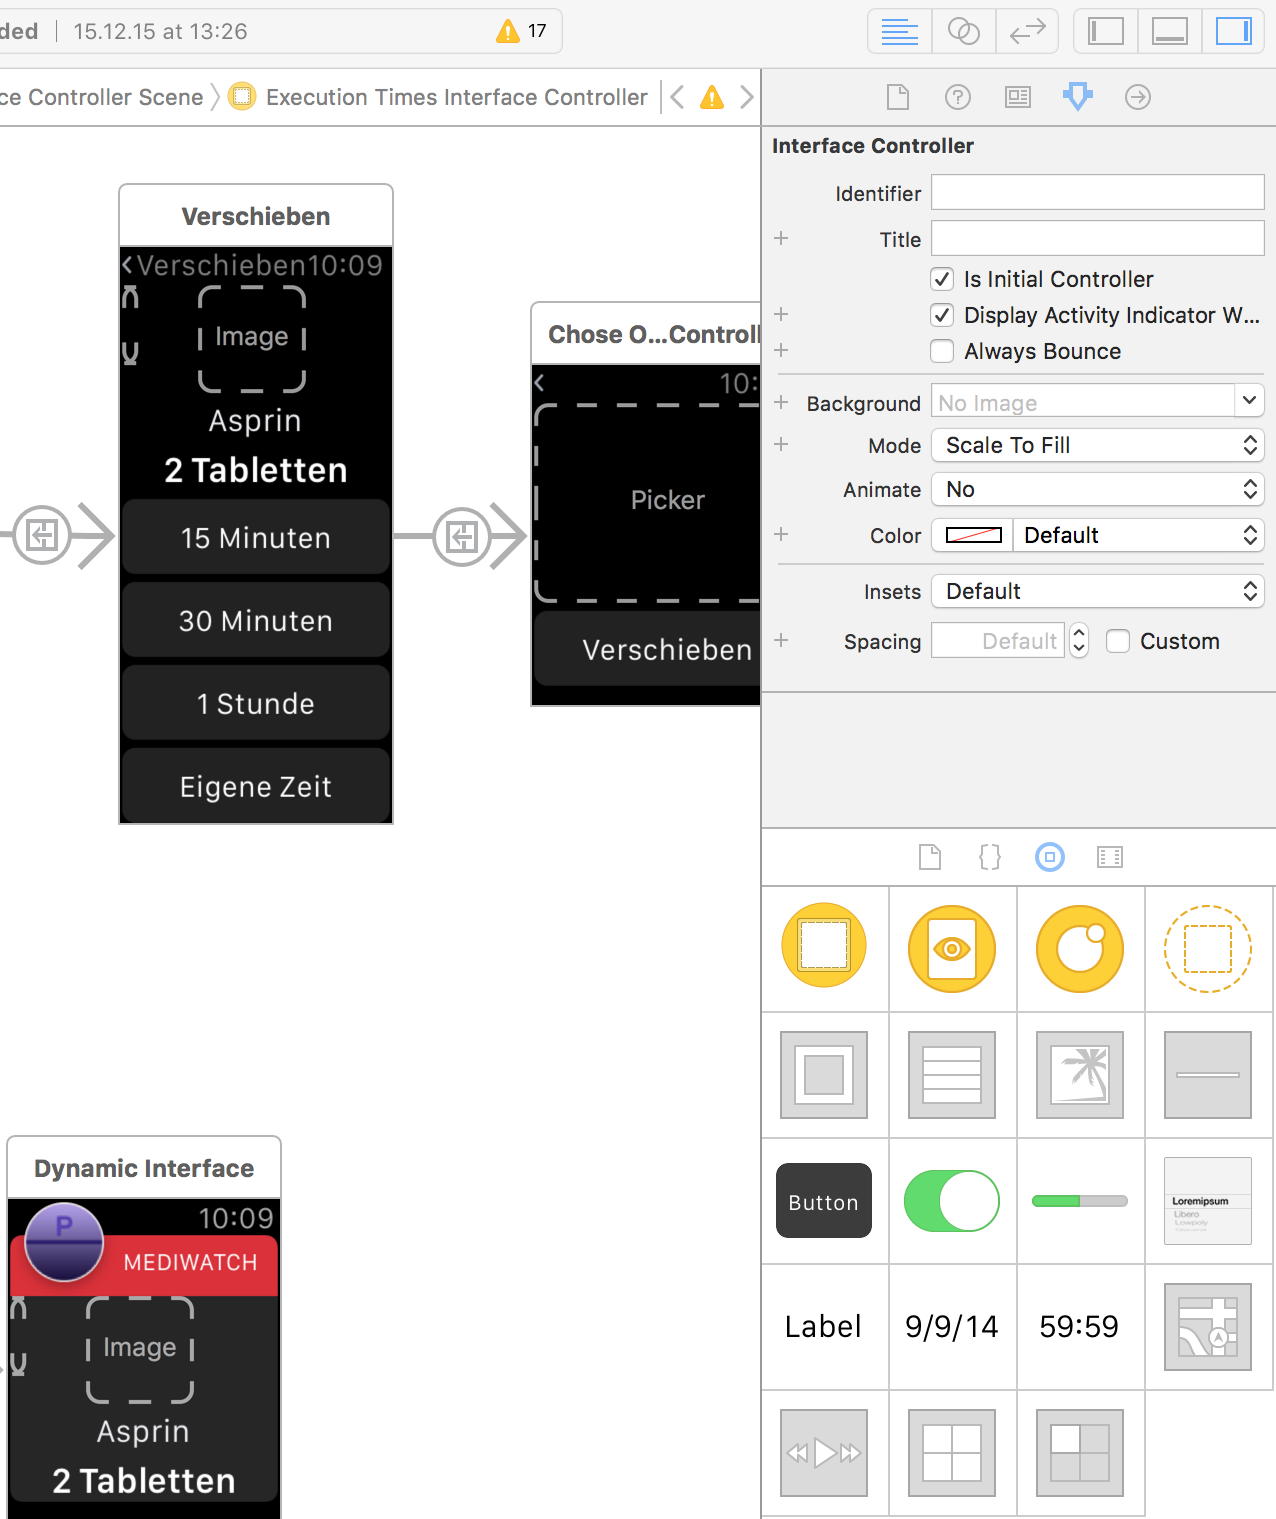
\includegraphics[width=0.9\textwidth]{04_realisation/screenshots/xcode-interface-elements}
\end{figure}

\begin{figure}
	\caption{Interface Elemente mit Quellcode verknüfen}
	\label{fig:xcode-interface-code-connect}
	\centering
	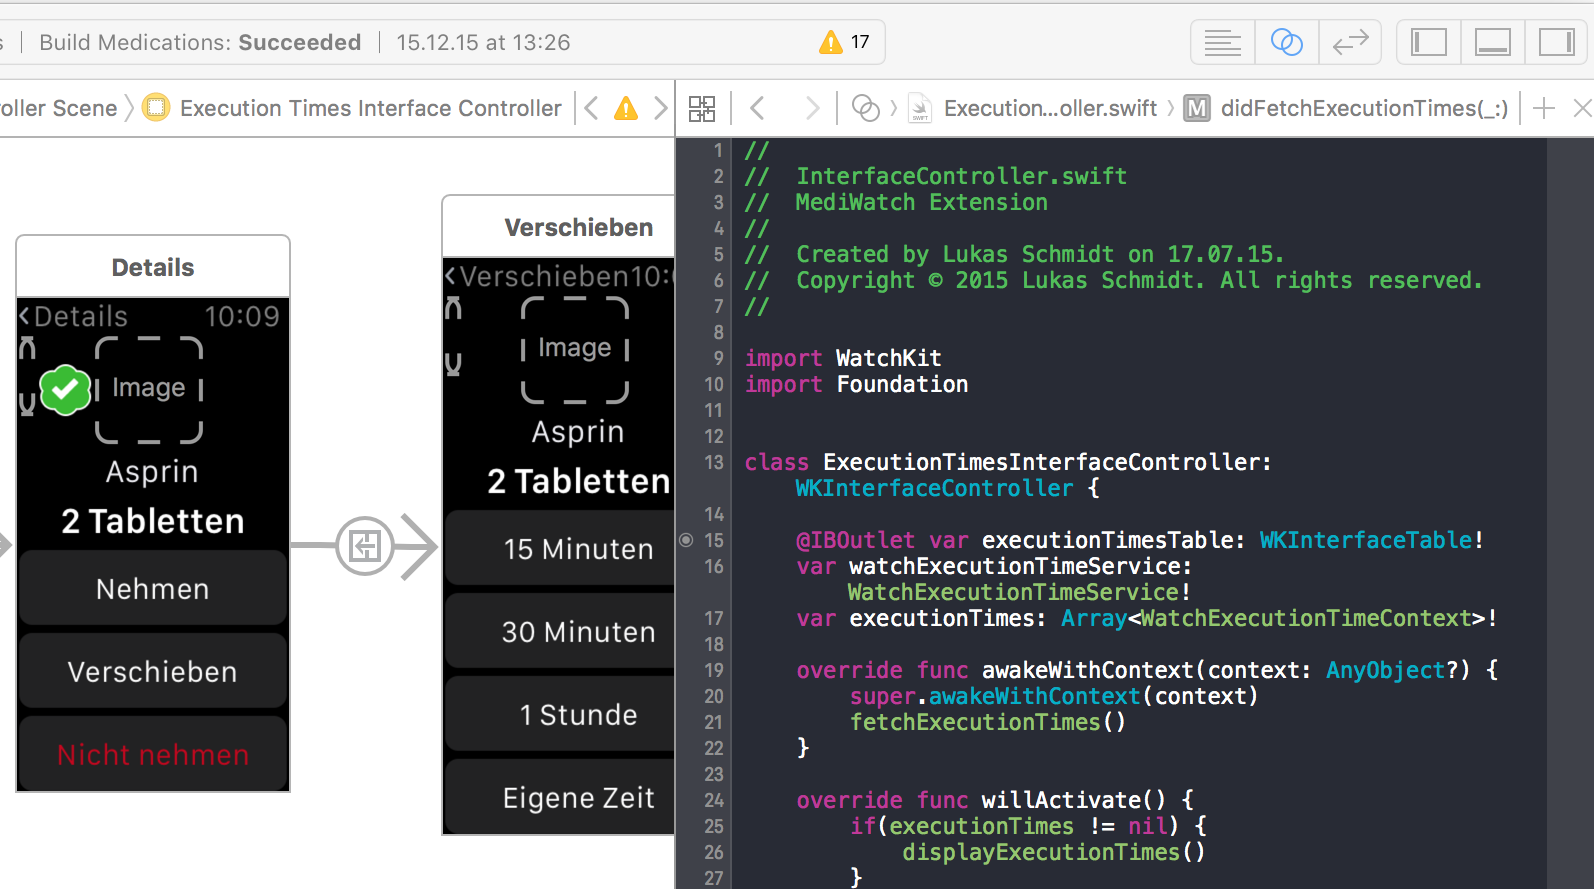
\includegraphics[width=0.9\textwidth]{04_realisation/screenshots/xcode-interface-code-connect}
\end{figure}

\section{WatchConnectivity}
Wichtig für die Kommunikation zwischen Uhr und iPhone ist das WatchConnectivity Framework. Hierbei ist ist im Listing xx zu sehen, wie genau eine Verbindung aufgebaut werden kann. Wichtig ist, das diese Verbindung zum richtigen Zeitpunkt im Application-Lifecycle aufgebaut wird, da es sonst zu Datenverlusten kommen kann. 

Mit der "sendMessage:" Methode können Nachrichten und Datenpakete gesendet werden, welche sich durch eine ID identifizieren lassen. Auch ist möglich eine direkte Antwort auf eine solche Nachricht über einen Replay-Handler zurück zu senden. So kann eine Art Request/Response Datentransfer realisiert werden. Zu beachten ist jedoch, dass die Kommunikation relativ langsam ist. Sie sollte nur verwendet werden um kleine Informationen zu senden.

Werden erst beim Watch-App Start benötigte Daten vom der iPhone angefordert, kann dies zu einer großen Verzögerung kommen. Daher sollten Informationen, die auf der Uhr angezeigt werden, nicht erst zum Zeitpunkt der Darstellung angefordert werden. Gibt es eine Datenänderung auf dem iPhone, die relevante Daten für die Uhr enthält, so sollten diese mit der Methode "transferUserInfo:" an die Uhr gesendet werden. Mit dem Aufrufen dieser Methode wird die übergebene Information nicht direkt zu Uhr geschickt. Das System sendet die Daten zu einem optimalen Zeitpunkt (starke Verbindung zur Uhr, mögliche WLAN Verbindung) an die Uhr. Wenn nun die Watch-App startet, so sind die Daten bereit und können direkt dargestellt werden.

Zum übertragen von größeren Daten steht die Methode "transferFile:" zur Verfügung. Die Methode verhält sich equivalent zu "transferUserInfo:", wird jedoch in der Realisierung nicht verwendet.

\section{Notification Management}
Notifications für die Medikationen werden mit der Notification API  registriert werden \cite{Apple:2015notif}. Auch kann das Verhalten der Notifications angepasst werden. So werden vordefinierte Aktionen wie "Einnehmen" oder "Verschieben" in die Notifications konfiguriert.

Bei der Notification handelt sich um eine UILocalNotification \cite{Apple:2015notif}. Die Art von Notification benötigt keinen Remote Server \todo{remote S. erklären}, sondern wird vom verbunden iPhone verwaltet. Zum jetzigen Zeitpunkt ist es nicht möglich UILocalNotification von der Uhr zu verwalten. Dies würde die Uhr im Falle der Mediwatch-Anwendung noch unabhängiger machen. Sind die Notifications einmal auf dem iPhone registriert, werden sie zum Ausführungszeitpunkt auf der Uhr angezeigt. Dazu ist keine Verbindung zum iPhone mehr nötig.

\section{Anwendung}

Die Anwendung besteht aus 2 Komponenten auf der Apple Watch. Eine native Notification  und eine auf der Uhr installierte und ausgeführte Anwendung (siehe \ref{ch:watch_software}).

\subsection{Notification}
 Die Notification bringt die Uhr zum Zeitpunkt der geplanten Medikamenteneinnahme zum vibrieren und lässt optional einen Ton erklingen. Dies führt dazu, dass der Anwender auf die Uhr Blick und die bevorstehende Medikamenteneinnahme bemerkt. Die Notification wurde darauf hin optimiert, dass eine große graphische Repräsentation des Medikaments angezeigt wird. Dem Nutzer wird so die Wiedererkennung des Medikaments zu erleichtert (siehe \ref{fig:watch-app-notification}).Neben dem Medikamentennamen wird auch die Dosierung des Medikaments dargestellt. Es wird dem Nutzer ermöglicht mit nur einer Aktion das Medikament zu Bestätigen oder es zu Verschieben. Die Notification ist darauf ausgelegt eine sehr schnelle Interaktion zu ermöglichen, damit der Nutzer nicht länger als 10 Sekunden mit der Uhr interagieren muss (siehe \ref{fig:watch-app-notification}).
 
\begin{figure}
	\caption{Notification für Medikament}
	\label{fig:watch-app-notification}
	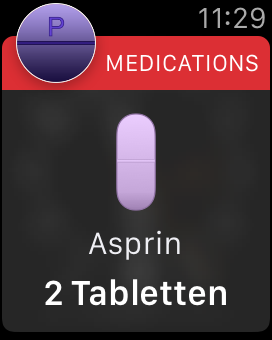
\includegraphics[width=0.5\textwidth]{04_realisation/screenshots/watch/notification01.png}
	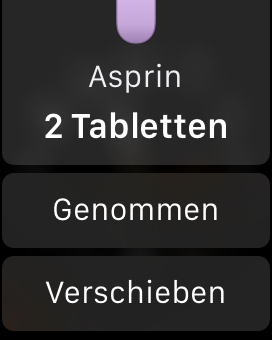
\includegraphics[width=0.5\textwidth]{04_realisation/screenshots/watch/notification02.png}
\end{figure}

\subsection{Native Anwendung}
Neben der Notification gibt es noch eine native App. Diese läuft auf der Uhr und stellt eine Liste der Medikamente des aktuellen Tages dar. Die App muss aktiv vom Nutzer gestartet werden. In \ref{fig:watch-app-take} wird ein Medikament aus der List ausgewählt. Nach dem man ein Medikament ausgewählt hat, bekommt man in einen Detailansicht des Medikaments zu sehen. Dort kann man nun das Medikament als genommen oder nicht genommen markieren. Ein visuelles Feedback zur Einnahme zeigt dem Nutzer seine Aktionen an. Von der Detailansicht ist es auch Möglich ein Medikament zur späteren Einnahme zu markieren. Hier hat der Anwender die Möglichkeit aus vordefinierten Zeiten auszuwählen oder eine eigene Zeit zu wählen (siehe \ref{fig:watch-app-delay}). 

\begin{figure}
	\caption{Native Anwendung: Interface zu wählen von eines Medikaments (oben links). Medikament als genommen bestätigen (oben rechts). Eigene Zeitdauer auswählen (unten links). Medikament ist in der Übersicht als verschoben markiert (unten rechts)}
	\label{fig:watch-app-take}
	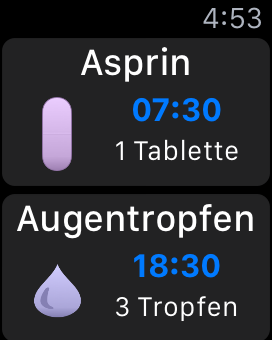
\includegraphics[width=0.5\textwidth]{04_realisation/screenshots/watch/notTaken01.png}
	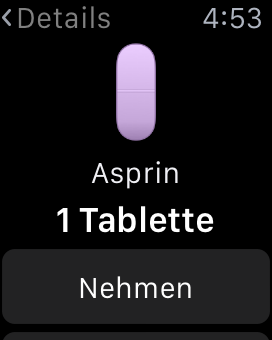
\includegraphics[width=0.5\textwidth]{04_realisation/screenshots/watch/notTaken02.png}
	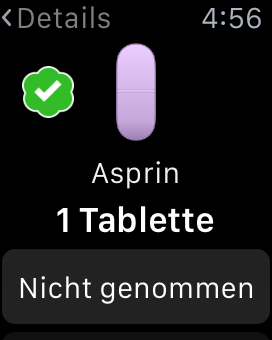
\includegraphics[width=0.5\textwidth]{04_realisation/screenshots/watch/taken01.png}
	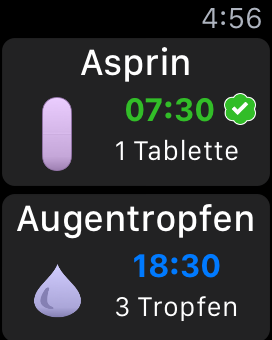
\includegraphics[width=0.5\textwidth]{04_realisation/screenshots/watch/taken02.png}
\end{figure}

\begin{figure}
	\caption{Native Anwendung: Interface zu verschieben von eines Medikaments (oben links). Zeitdauer für das Verschiebenwählen (oben rechts). Medikament ist als genommen markiert (unten links). Medikament ist in der Übersicht als genommen markiert(unten rechts)}
	\label{fig:watch-app-delay}
	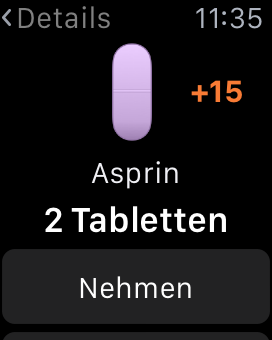
\includegraphics[width=0.5\textwidth]{04_realisation/screenshots/watch/delay01.png}
	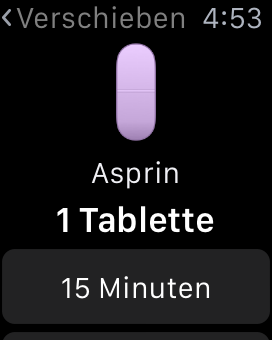
\includegraphics[width=0.5\textwidth]{04_realisation/screenshots/watch/delay02.png}
	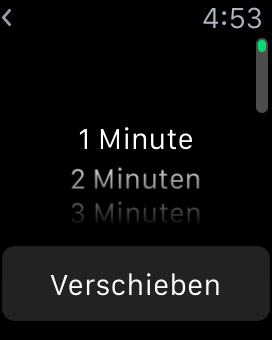
\includegraphics[width=0.5\textwidth]{04_realisation/screenshots/watch/delay03.png}
	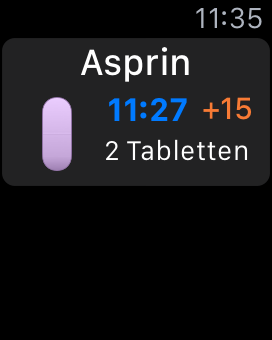
\includegraphics[width=0.5\textwidth]{04_realisation/screenshots/watch/delay04.png}
\end{figure}


